Für die Aufgabe werden die folgenden Bauteile benötigt, wobei für das Tastenfeld eine 4x4 Matrix aus Tastern benutzt werden kann, welche ähnlich zu dem Schaltplan sind:

\begin{itemize}
    \item Arduino UNO (im weiteren nur noch Arduino genannt)
    \item RGB LED
    \item 3x 470-Ohm Widerstände
    \item 4x4 Tastenfeld
    \item Jumper-Kabel zum Verbinden
    \item USB Kabel für Debug und Datenaustausch
\end{itemize}

Der Arduino ist ein Mikrocontroller auf Basis des ATmega328P. Er verfügt über 14 digitale Ein-/Ausgangspins, 6 analoge Eingänge, einen 16-MHz-Keramikresonator, einen USB-Anschluss, eine Netzbuchse, einen ICSP-Header und einen Reset-Knopf \cite{online:arduino}.

Die RGB LED enspricht einer kleinen 5mm LED, welche rotes, blaues und grünes Licht abstrahlen kann. Diese LED wird zur Signalisierung der Zustände des Nummernschlosses benötigt. Die Vorwiderstände von 470 Ohm werden zum Schutz der Dioden verwendet, da der Arduino eine Ausgangsspannung von 5V der GPIO-Pins hat. 

\subsection{Funktionsweise des Tastenfeldes}

Das 4x4 Tastenfeld ist ein 16/8 Multiplexer. Es werden anstelle von 16 Pins, 8 Pins auf dem Aruduino benötigt. Dabei sind 4 Pins Ausgänge (R1-R4) und 4 Pins Eingänge (C1-C4). Auf Abbildung \ref{fig:schematic} ist der Schaltplan des Tastenfeldes abgebildet. Um eine gedrückte Taste zu ermitteln werden alle Ausgänge hintereinander auf High gesetzt währenddessen geprüft wird ob eine der Eingänge auf High ist. Sind Eingang und Ausgang auf High, ist somit automatisch die gedrückte Taste bekannt. 

\begin{figure}[H]
    \caption{4x4 Tastenfeld - Schaltplan}
    \centering
    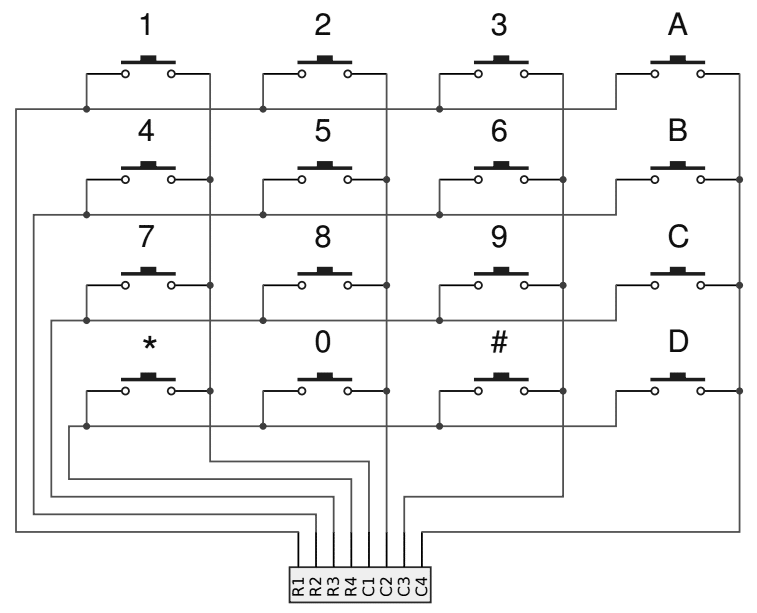
\includegraphics[width=0.6\textwidth]{images/4x4-keypad.png}
    \label{fig:schematic}
\end{figure}

\subsection{Pinbelegung des Arudinos}

Das 4x4 Tastenfeld und die RGB LED werden mit dem Arduino über folgende GPIO Pins verbunden:
\begin{lstlisting}[style=CStyle]
const int Output[rows]={2,3,4,5};
const int Input[columns]={6,7,8,9};
const int redPin = 10;
const int greedPin = 11;
const int bluePin = 12;
\end{lstlisting}

Dabei werden GPIO Pin 2 bis 5 als digitaler Output festgelegt. Diese Pins entsprechen R1 bis R4 des Tastenfelds. GPIO 6 bis 9 sind als digitaler Input eingestellt und entsprechen C1 bis C4. GPIO Pin 10 bis 12 sind digitale Ausgänge um die Intensität der jeweiligen Farben einzustellen.

\subsection{Versuchsaufbau}

Abbildung \ref{fig:sketch} ist der Sketch des Zahlenschlosses. Hierbei sind der Arduino-Uno, die RGB-LED, die Vorwiderstände und das Tastenfeld korrekt verbunden. Dabei stimmen die Pin-Belegungen mit dem aus dem Quellcode verwendeten Pins überein. 

\begin{figure}[H]
    \caption{Sketch des Zahlenschlosses}
    \centering
    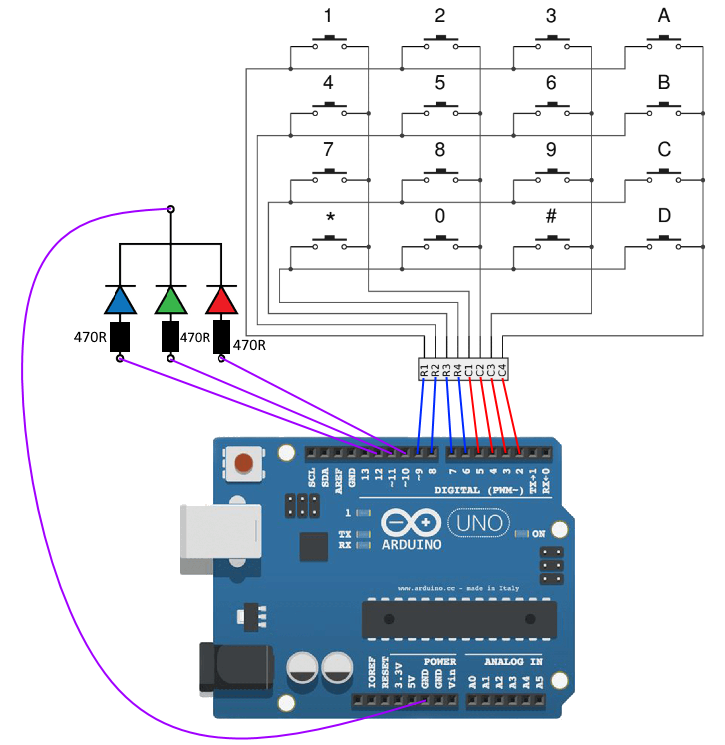
\includegraphics[width=0.7\textwidth]{images/sketch.png}
    \label{fig:sketch}
\end{figure}

\subsection{Zustandsmaschine}

Das Verhalten des Nummernschlosses wird als eine Zustandsmaschine beschrieben, welche in Abbildung \ref{fig:M1} zu sehen ist. Die PIN und der PUK werden im Quellcode fest definiert. Der Zustand 'init' ist der Startzustand der Maschine. Sobald eine Taste gedrückt wird, wechselt der Zustand in 'key'. Hierbei werden die Eingaben mitgezählt, bei der korrekten Eingabe einer Stelle wird der Zähler erhöht ('right key'). Ist die Eingabe falsch, wird zurück in den 'init' Zustand gewechselt und die Eingabe zurückgesetzt. Nach 4 Fehleingaben wird das Schloss gesperrt und von 'key' in den Zustand 'locked' gewechselt. Dieser Zustand kann nur verlassen werden, wenn die PUK korrekt eingegeben wird. Ist die PIN korrekt, wird in den Zustand 'open' gewechselt und das Schloss ist geöffnet. Hierbei kann der PIN geändert werden oder das Schloss sperrt sich nach einer gewissen Zeitspanne automatisch und wechselt in den Zustand 'init'. Falls eine PIN-Änderung gewünscht wird, muss eine bestimmte Zeichenfolge eingegeben werden. Nach der Aufzeichnung der Eingaben wird der neue PIN gespeichert und es wird zurück in den 'open' Zustand gewechselt. 

\begin{figure}[H]
\caption{Zustandsmaschine der Schlosssteuerun} \label{fig:M1}
\centering
    \begin{tikzpicture}[shorten >=1pt,node distance=3cm,on grid]
      \node[state,initial]   (init)                {init};
      \node[state]           (key) [right=of init] {key};
      \node[state]           (locked) [right=of key] {locked};
      \node[state]           (open) [right=of locked] {open};
      \node[state]           (change) [right=of open] {change};
      \path[->] (init)   edge   node [below] {input} (key)
                (key)    edge  [bend right]  node [above]   {wrong input} (init)
                         edge  [bend left]  node [above]   {correct pin} (open)
                         edge  [loop below]  node           {right key} ()
                         edge  node [below] {tries > 4} (locked)
                (locked) edge  [bend left=75]  node [below] {unlock with puk} (init)
                (open)   edge  [bend left]  node [above] {input} (change)
                         edge  [bend right=75]  node [below] {timeout} (init)
                (change) edge  [loop below]  node {key input} ()
                         edge [bend left=45] node [below] {change command} (open);
    \end{tikzpicture}
\end{figure}

Die Abbildung \ref{fig:usecase} ist ein Anwendungsfalldiagramm für die Schlosssteuerung. Hierbei gibt es zwei Gruppen von Anwendern. Die erste Gruppe sind die nutzenden Personen ('Employee'), welche die Tür entsperren wollen um durchzugehen. Diese benötigen hierfür einen PIN. Die zweite Gruppe sind die Administratoren, welche sich um die Verwaltung kümmern. Die Administratoren können gesperrte Schlösser mit der Hilfe eines PUK entsperren. Zusätzlich können sie den PIN ändern, wenn das Schloss offen ist und sie einen Befehl auf dem Tastenfeld eingeben. 

\begin{figure}[H]
    \caption{Use-Case Diagramm}
    \centering
    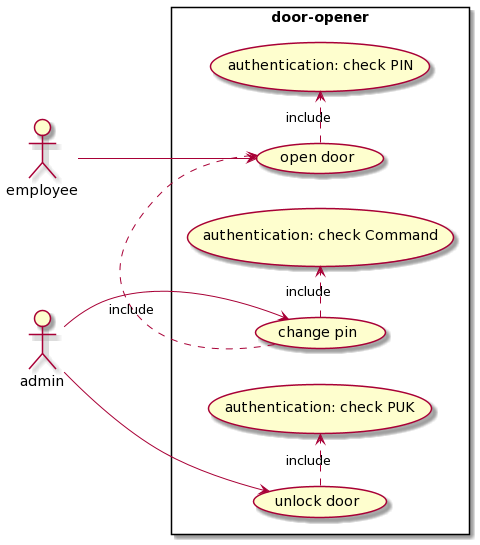
\includegraphics[width=0.5\textwidth]{images/usecase.png}
    \label{fig:usecase}
\end{figure}

In Abbildung \ref{fig:sequence-user} wird eine Sequenz von nutzenden Personen ('Employee'), Türschloss ('Keypad') und Tür ('Door') gezeigt. Zum besseren Verständnis wurde die Tür als Objekt noch zusätzlich eingefügt, auch wenn diese nicht im Aufbau erklärt wird. Möchte die nutzende Person die Tür öffnen gibt es zwei Fälle. Wenn das Schloss nicht gesperrt ist, kann die nutzende Person einen PIN eingeben um die Tür zu entsperren. Dabei werden die Antworten des Türschlosses als Farben auf der LED visualisiert (siehe Kapitel \ref{state-colors}). Ist die Tür gesperrt, kann die nutzende Person zwar das Tasten klicken aber das Schloss wird nicht reagieren.

\begin{figure}[H]
    \caption{Sequenzdiagramm - nutzende Person}
    \centering
    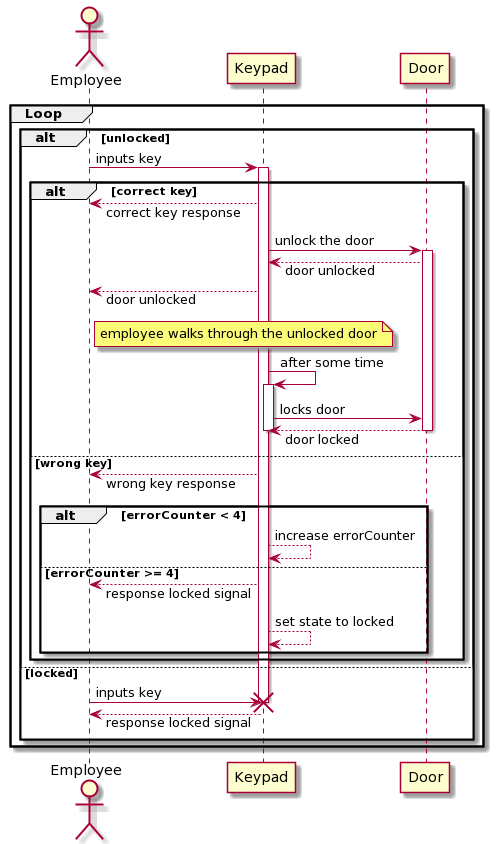
\includegraphics[width=0.6\textwidth]{images/sequence-user.png}
    \label{fig:sequence-user}
\end{figure}

Nun wird in der Abbildung \ref{fig:sequence-admin} die Sequenz von administrierenden Personen ('Admin') und dem Türschloss beschrieben. Dabei wird auf die Möglichkeit eingegangen das Schloss zu entsperren, falls der PIN zu oft falsch eingegeben wurde. Zusätzlich wird auch die Möglichkeit der Änderung des PIN beschrieben. In diesem Fall muss das Türschloss bereits über den PIN geöffnet worden sein. Auch hier werden die Antworten des Türschlosses mit Hilfe der LED visualisiert (siehe Kapitel \ref{state-colors}).

\begin{figure}[H]
    \caption{Sequenzdiagramm - Administrator}
    \centering
    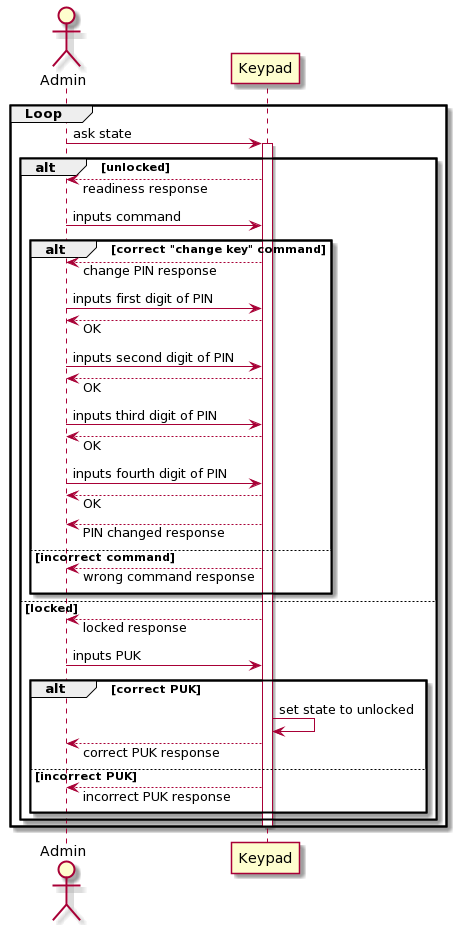
\includegraphics[width=0.6\textwidth]{images/sequence-admin.png}
    \label{fig:sequence-admin}
\end{figure}